\documentclass[tikz,border=0pt]{standalone}
\usepackage{amsmath, amssymb}
\usetikzlibrary{matrix, positioning, fit, backgrounds, calc}
\usepackage{helvet}
\usepackage{avant}
\renewcommand*\familydefault{\sfdefault}
\usepackage{textcomp}

\usepackage{fontspec}
\setmainfont{TeX Gyre Termes}
\setsansfont[
Path = fonts/,
UprightFont = *Medium.ttf,
BoldFont    = *Bold.ttf,
AutoFakeSlant = 0.2
]{GmarketSansTTF}
\begin{document}
	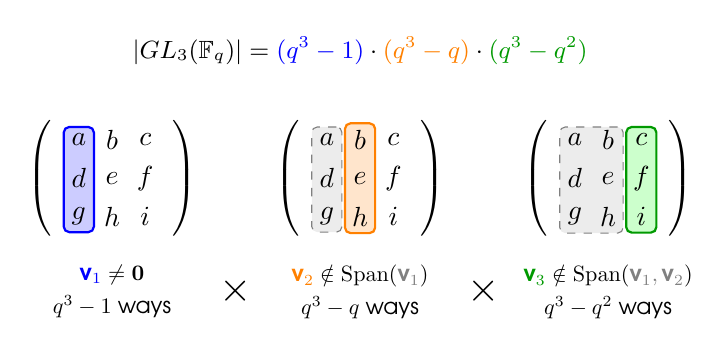
\begin{tikzpicture}[
		font=\sffamily,
		% Style for the matrices
		mtx/.style={
			matrix of math nodes,
			left delimiter=(, right delimiter=),
			nodes={minimum width=1em, inner sep=2pt, anchor=center},
			column sep=2pt, row sep=2pt,
			ampersand replacement=\&
		},
		% Highlighting styles for active columns
		hl-v1/.style={fill=blue!20, draw=blue, thick, rounded corners=2pt, inner sep=.25pt},
		hl-v2/.style={fill=orange!20, draw=orange, thick, rounded corners=2pt, inner sep=.25pt},
		hl-v3/.style={fill=green!20, draw=green!60!black, thick, rounded corners=2pt, inner sep=.25pt},
		hl-v4/.style={fill=purple!20, draw=purple, thick, rounded corners=2pt, inner sep=.25pt},
		% Style for the accumulating "Span Box"
		hl-span/.style={fill=gray!15, draw=gray, dashed, rounded corners=2pt, inner sep=.25pt},
		% Title & Text
		mainTitle/.style={font=\sffamily\bfseries\LARGE, color=darkgray, align=center},
		term label/.style={font=\bfseries\small, align=center}
		]
		
		% ==============================================================================
		% ROW 2: m = 3 (Scaling Up)
		% ==============================================================================
		\begin{scope}[shift={(-3, 0)}, scale=0.9]
			\node[term label] at (3.5, 1.8) {$|GL_3(\mathbb F_q)| = \textcolor{blue}{(q^3-1)} \cdot \textcolor{orange}{(q^3-q)} \cdot \textcolor{green!60!black}{(q^3-q^2)}$};
			
			% Column 1
			\matrix[mtx] (M3_1) at (0, 0) {
					a \& b \& c \\
					d \& e \& f \\
					g \& h \& i \\
				};
			\begin{scope}[on background layer] \node[hl-v1, fit=(M3_1-1-1)(M3_1-3-1)] {}; \end{scope}
			\node[below=0.2cm of M3_1, align=center, scale=0.8] {
					$\textcolor{blue}{\textbf{v}_1} \neq \mathbf{0}$ \\[1mm]
					\textbf{$q^3 - 1$} ways
				};
			
			% Column 2
			\matrix[mtx] (M3_2) at (3.5, 0) {
					a \& b \& c \\
					d \& e \& f \\
					g \& h \& i \\
				};
			\begin{scope}[on background layer]
					\node[hl-span, fit=(M3_2-1-1)(M3_2-3-1)] {}; % v1 forbidden
					\node[hl-v2, fit=(M3_2-1-2)(M3_2-3-2)] {};
				\end{scope}
			\node[below=0.2cm of M3_2, align=center, scale=0.8] {
					$\textcolor{orange}{\textbf{v}_2} \notin \mathrm{Span}(\textcolor{gray}{\textbf{v}_1})$ \\[1mm]
					\textbf{$q^3 - q$} ways
				};
			
			% Column 3
			\matrix[mtx] (M3_3) at (7, 0) {
					a \& b \& c \\
					d \& e \& f \\
					g \& h \& i \\
				};
			\begin{scope}[on background layer]
					\node[hl-span, fit=(M3_3-1-1)(M3_3-3-2)] {}; % v1, v2 forbidden
					\node[hl-v3, fit=(M3_3-1-3)(M3_3-3-3)] {};
				\end{scope}
			\node[below=0.2cm of M3_3, align=center, scale=0.8] {
					$\textcolor{green!60!black}{\textbf{v}_3} \notin \mathrm{Span}(\textcolor{gray}{\textbf{v}_1, \textbf{v}_2})$ \\[1mm]
					\textbf{$q^3 - q^2$} ways
				};
			
			% Draw multiplication signs after nodes exist
			\node[scale=1.5] at ($(M3_1)!0.5!(M3_2)+(0,-1.6)$) {$\times$};
			\node[scale=1.5] at ($(M3_2)!0.5!(M3_3)+(0,-1.6)$) {$\times$};
		\end{scope}
	\end{tikzpicture}
\end{document}